\documentclass{ximera}

 

\usepackage{epsfig}

\graphicspath{
  {./}
  {figures/}
}

\usepackage{morewrites}
\makeatletter
\newcommand\subfile[1]{%
\renewcommand{\input}[1]{}%
\begingroup\skip@preamble\otherinput{#1}\endgroup\par\vspace{\topsep}
\let\input\otherinput}
\makeatother

\newcommand{\includeexercises}{\directlua{dofile("/home/jim/linearAlgebra/laode/exercises.lua")}}

%\newcounter{ccounter}
%\setcounter{ccounter}{1}
%\newcommand{\Chapter}[1]{\setcounter{chapter}{\arabic{ccounter}}\chapter{#1}\addtocounter{ccounter}{1}}

%\newcommand{\section}[1]{\section{#1}\setcounter{thm}{0}\setcounter{equation}{0}}

%\renewcommand{\theequation}{\arabic{chapter}.\arabic{section}.\arabic{equation}}
%\renewcommand{\thefigure}{\arabic{chapter}.\arabic{figure}}
%\renewcommand{\thetable}{\arabic{chapter}.\arabic{table}}

%\newcommand{\Sec}[2]{\section{#1}\markright{\arabic{ccounter}.\arabic{section}.#2}\setcounter{equation}{0}\setcounter{thm}{0}\setcounter{figure}{0}}

\newcommand{\Sec}[2]{\section{#1}}

\setcounter{secnumdepth}{2}
%\setcounter{secnumdepth}{1} 

%\newcounter{THM}
%\renewcommand{\theTHM}{\arabic{chapter}.\arabic{section}}

\newcommand{\trademark}{{R\!\!\!\!\!\bigcirc}}
%\newtheorem{exercise}{}

\newcommand{\dfield}{{\sf dfield9}}
\newcommand{\pplane}{{\sf pplane9}}

\newcommand{\EXER}{\section*{Exercises}}%\vspace*{0.2in}\hrule\small\setcounter{exercise}{0}}
\newcommand{\CEXER}{}%\vspace{0.08in}\begin{center}Computer Exercises\end{center}}
\newcommand{\TEXER}{} %\vspace{0.08in}\begin{center}Hand Exercises\end{center}}
\newcommand{\AEXER}{} %\vspace{0.08in}\begin{center}Hand Exercises\end{center}}

% BADBAD: \newcommand{\Bbb}{\bf}

\newcommand{\R}{\mbox{$\Bbb{R}$}}
\newcommand{\C}{\mbox{$\Bbb{C}$}}
\newcommand{\Z}{\mbox{$\Bbb{Z}$}}
\newcommand{\N}{\mbox{$\Bbb{N}$}}
\newcommand{\D}{\mbox{{\bf D}}}
\usepackage{amssymb}
%\newcommand{\qed}{\hfill\mbox{\raggedright$\square$} \vspace{1ex}}
%\newcommand{\proof}{\noindent {\bf Proof:} \hspace{0.1in}}

\newcommand{\setmin}{\;\mbox{--}\;}
\newcommand{\Matlab}{{M\small{AT\-LAB}} }
\newcommand{\Matlabp}{{M\small{AT\-LAB}}}
\newcommand{\computer}{\Matlab Instructions}
\newcommand{\half}{\mbox{$\frac{1}{2}$}}
\newcommand{\compose}{\raisebox{.15ex}{\mbox{{\scriptsize$\circ$}}}}
\newcommand{\AND}{\quad\mbox{and}\quad}
\newcommand{\vect}[2]{\left(\begin{array}{c} #1_1 \\ \vdots \\
 #1_{#2}\end{array}\right)}
\newcommand{\mattwo}[4]{\left(\begin{array}{rr} #1 & #2\\ #3
&#4\end{array}\right)}
\newcommand{\mattwoc}[4]{\left(\begin{array}{cc} #1 & #2\\ #3
&#4\end{array}\right)}
\newcommand{\vectwo}[2]{\left(\begin{array}{r} #1 \\ #2\end{array}\right)}
\newcommand{\vectwoc}[2]{\left(\begin{array}{c} #1 \\ #2\end{array}\right)}

\newcommand{\ignore}[1]{}


\newcommand{\inv}{^{-1}}
\newcommand{\CC}{{\cal C}}
\newcommand{\CCone}{\CC^1}
\newcommand{\Span}{{\rm span}}
\newcommand{\rank}{{\rm rank}}
\newcommand{\trace}{{\rm tr}}
\newcommand{\RE}{{\rm Re}}
\newcommand{\IM}{{\rm Im}}
\newcommand{\nulls}{{\rm null\;space}}

\newcommand{\dps}{\displaystyle}
\newcommand{\arraystart}{\renewcommand{\arraystretch}{1.8}}
\newcommand{\arrayfinish}{\renewcommand{\arraystretch}{1.2}}
\newcommand{\Start}[1]{\vspace{0.08in}\noindent {\bf Section~\ref{#1}}}
\newcommand{\exer}[1]{\noindent {\bf \ref{#1}}}
\newcommand{\ans}{}
\newcommand{\matthree}[9]{\left(\begin{array}{rrr} #1 & #2 & #3 \\ #4 & #5 & #6
\\ #7 & #8 & #9\end{array}\right)}
\newcommand{\cvectwo}[2]{\left(\begin{array}{c} #1 \\ #2\end{array}\right)}
\newcommand{\cmatthree}[9]{\left(\begin{array}{ccc} #1 & #2 & #3 \\ #4 & #5 &
#6 \\ #7 & #8 & #9\end{array}\right)}
\newcommand{\vecthree}[3]{\left(\begin{array}{r} #1 \\ #2 \\
#3\end{array}\right)}
\newcommand{\cvecthree}[3]{\left(\begin{array}{c} #1 \\ #2 \\
#3\end{array}\right)}
\newcommand{\cmattwo}[4]{\left(\begin{array}{cc} #1 & #2\\ #3
&#4\end{array}\right)}

\newcommand{\Matrix}[1]{\ensuremath{\left(\begin{array}{rrrrrrrrrrrrrrrrrr} #1 \end{array}\right)}}

\newcommand{\Matrixc}[1]{\ensuremath{\left(\begin{array}{cccccccccccc} #1 \end{array}\right)}}



\renewcommand{\labelenumi}{\theenumi)}
\newenvironment{enumeratea}%
{\begingroup
 \renewcommand{\theenumi}{\alph{enumi}}
 \renewcommand{\labelenumi}{(\theenumi)}
 \begin{enumerate}}
 {\end{enumerate}\endgroup}



\newcounter{help}
\renewcommand{\thehelp}{\thesection.\arabic{equation}}

%\newenvironment{equation*}%
%{\renewcommand\endequation{\eqno (\theequation)* $$}%
%   \begin{equation}}%
%   {\end{equation}\renewcommand\endequation{\eqno \@eqnnum
%$$\global\@ignoretrue}}

%\input{psfig.tex}

\author{Martin Golubitsky and Michael Dellnitz}

%\newenvironment{matlabEquation}%
%{\renewcommand\endequation{\eqno (\theequation*) $$}%
%   \begin{equation}}%
%   {\end{equation}\renewcommand\endequation{\eqno \@eqnnum
% $$\global\@ignoretrue}}

\newcommand{\soln}{\textbf{Solution:} }
\newcommand{\exercap}[1]{\centerline{Figure~\ref{#1}}}
\newcommand{\exercaptwo}[1]{\centerline{Figure~\ref{#1}a\hspace{2.1in}
Figure~\ref{#1}b}}
\newcommand{\exercapthree}[1]{\centerline{Figure~\ref{#1}a\hspace{1.2in}
Figure~\ref{#1}b\hspace{1.2in}Figure~\ref{#1}c}}
\newcommand{\para}{\hspace{0.4in}}

\renewenvironment{solution}{\suppress}{\endsuppress}

\ifxake
\newenvironment{matlabEquation}{\begin{equation}}{\end{equation}}
\else
\newenvironment{matlabEquation}%
{\let\oldtheequation\theequation\renewcommand{\theequation}{\oldtheequation*}\begin{equation}}%
  {\end{equation}\let\theequation\oldtheequation}
\fi

\makeatother


\title{The Geometry of Vector Operations}

\begin{document}
\begin{abstract}
\end{abstract}
\maketitle


\label{S:1.4}

In this section we discuss the geometry of addition, scalar
multiplication, and dot product of vectors.  We also use \Matlab
graphics to visualize these operations.


\subsection*{Geometry of Addition} \index{vector!addition}

\Matlab has an excellent graphics language that we shall use
at various times to illustrate concepts in both two and three
dimensions.  In order to make the connections between ideas and
graphics more transparent, we will sometimes use previously
developed \Matlab programs.  We begin with such an example ---
the illustration of the parallelogram law\index{parallelogram law}
for vector addition\index{vector!addition}.

Suppose that $x$ and $y$ are two planar vectors.  Think of these
vectors as line segments from the origin to the points $x$ and
$y$ in $\R^2$. We use a program written by T.A. Bryan to
visualize $x+y$.  In \Matlab type\footnote{Note that all \Matlab
commands are case sensitive --- upper and lower case must be correct}:
\begin{verbatim}
x = [1 2];
y = [-2 3];
addvec(x,y)
\end{verbatim}  \index{\computer!addvec}
The vector $x$ is displayed in blue, the vector $y$ in green,
and the vector $x+y$ in red.  Note that $x+y$ is just the diagonal
of the parallelogram spanned by $x$ and $y$.  A black and white
version of this figure is given in Figure~\ref{F:vec2}.

\begin{figure}[htb]
         \centerline{%
         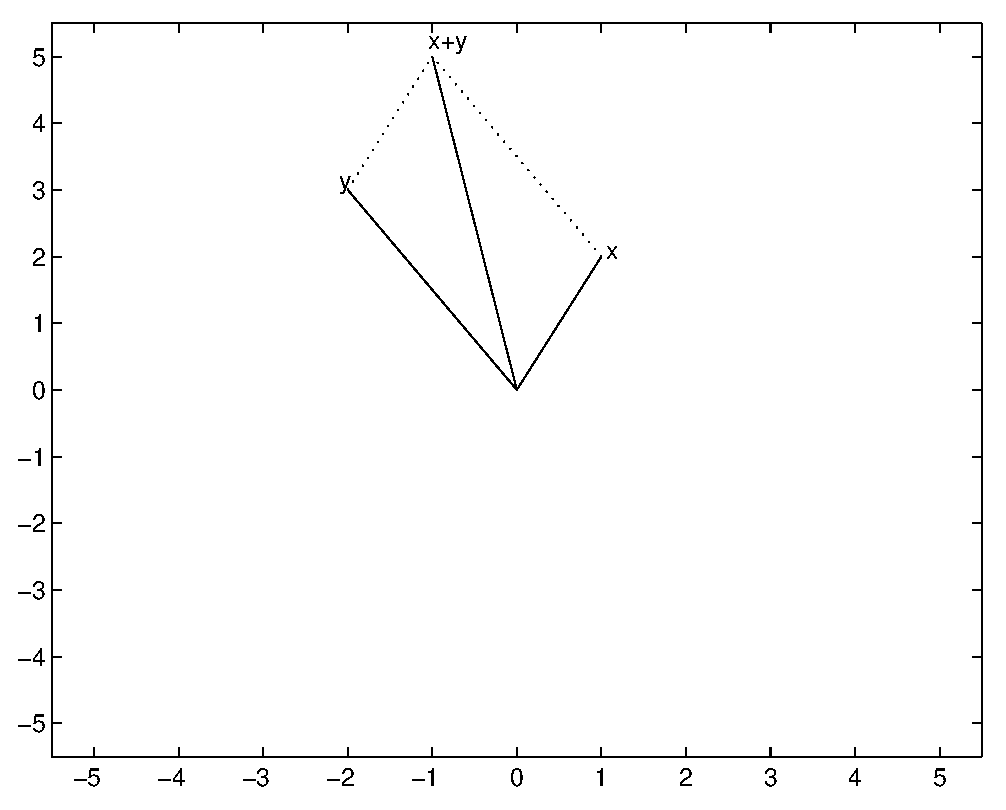
\psfig{file=../figures/vec2.eps,width=2.5in}}
         \caption{Addition of two planar vectors.}
         \label{F:vec2}
\end{figure}


The parallelogram law (the diagonal of the parallelogram spanned
by $x$ and $y$ is $x+y$) is equally valid in three dimensions.
Use \Matlab to verify this statement by typing:
\begin{verbatim}
x = [1 0 2];
y = [-1 4 1];
addvec3(x,y)
\end{verbatim} \index{\computer!addvec3}
The parallelogram spanned by $x$ and $y$ in $\R^3$ is shown in
cyan; the diagonal $x+y$ is shown in blue.  See Figure~\ref{F:vec3}.   
To test your geometric intuition, make several choices of vectors $x$ and
$y$.  Note that one vertex of the parallelogram is always the
origin.

\begin{figure}[htb]
         \centerline{%
         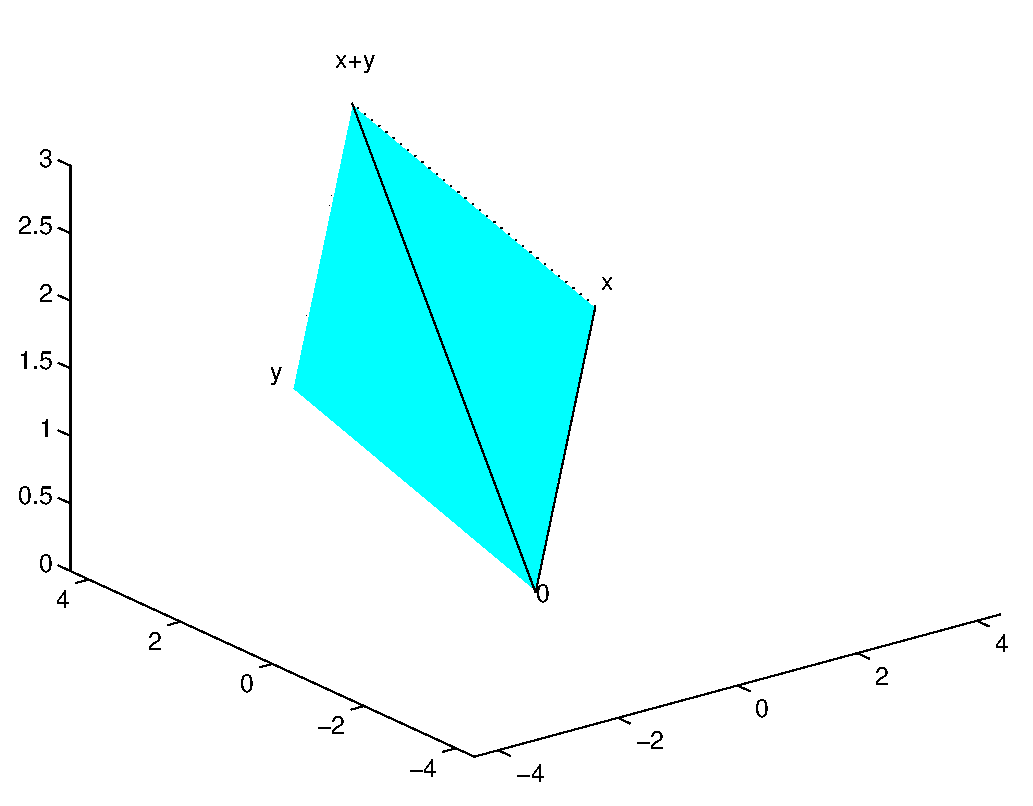
\psfig{file=../figures/vec3.eps,width=3.0in}}
         \caption{Addition of two vectors in three dimensions.}
         \label{F:vec3}
\end{figure}


\subsection*{Geometry of Scalar Multiplication}

In all dimensions scalar multiplication\index{scalar
multiplication} just scales the length of the vector.  To
discuss this point we need to define the length of a vector.
View an $n$-vector $x=(x_1,\ldots,x_n)$ as a line segment from
the origin to the point $x$.  Using the Pythagorean theorem, it can
be shown that the {\em length\/}\index{length}\index{vector!length} 
or {\em norm\/}\index{norm}\index{vector!norm} of this line segment is:
\[
||x||  = \sqrt{x_1^2 + \cdots + x_n^2}.
\] \index{\computer:$||\cdot|| $}
\Matlab has the command {\tt norm} for finding the length of a
vector.  Test this by entering the $3$-vector
\begin{verbatim}
x = [1 4 2];
\end{verbatim}
Then type
\begin{verbatim}
norm(x)
\end{verbatim}  \index{\computer!norm}
\Matlab responds with:
\begin{verbatim}
ans =
    4.5826
\end{verbatim}
which is indeed approximately $\sqrt{1+4^2+2^2} = \sqrt{21}$.

Now suppose $r\in\R$ and $x\in\R^n$.  A calculation shows that
\begin{equation}  \label{E:lengths}
||rx||  = |r| ||x||.
\end{equation}
See Exercise~\ref{c1.4.9A}.  Note also that if $r$ is positive, 
then the direction of $rx$
is the same as that of $x$; while if $r$ is negative, then the
direction of $rx$ is opposite to the direction of $x$.  The
lengths of the vectors $3x$ and $-3x$ are each three times the
length of $x$ --- but these vectors point in opposite
directions.  Scalar multiplication by the scalar $0$ produces
the $0$ vector, the vector whose entries are all zero.

\subsection*{Dot Product and Angles}

The {\em dot product\/}\index{dot product} of two $n$-vectors
$x=(x_1,\ldots,x_n)$ and $y=(y_1,\ldots,y_n)$ is an important
operation on vectors.  It is defined by:
\begin{equation}  \label{e:dotproduct}
x\cdot y = x_1y_1 + \cdots + x_ny_n.
\end{equation}
Note that $x\cdot x$ is just $||x||^2$, the length of $x$
squared.

\Matlab also has a command for computing dot products of
$n$-vectors.  Type
\begin{verbatim}
x = [1 4 2];
y = [2 3 -1];
dot(x,y)
\end{verbatim}\index{\computer!dot}
\Matlab responds with the dot product of $x$ and $y$, namely,
\begin{verbatim}
ans =
    12
\end{verbatim}

One of the most important facts concerning dot products is the
one that states
\begin{equation} \label{dotprod=0}
x\cdot y = 0 \quad \mbox{if and only if} \quad \mbox{$x$ and $y$
are perpendicular}.
\end{equation}  \index{perpendicular}
Indeed, dot product also gives a way of numerically determining
the angle between $n$-vectors, as follows.
\begin{theorem} \label{T:dotangle}
Let $\theta$ be the angle between two nonzero $n$-vectors $x$
and $y$.  Then
\begin{equation}  \label{e:dotproductang}
\cos \theta = \frac{x\cdot y}{||x|| ||y||}.
\end{equation}
\end{theorem}
It follows that $\cos \theta=0$
if and only if $x\cdot y = 0$.  Thus \eqref{dotprod=0} is valid.

\begin{proof}  Theorem~\ref{T:dotangle} is just a restatement of the
{\em law of cosines\/}\index{law of cosines}.  Recall that the
law of cosines states that
\[
c^2 = a^2 + b^2 -2ab\cos\theta,
\]
where $a,b,c$ are the lengths of the sides of a triangle and $\theta$
is the interior angle opposite the side of length $c$.
In vector notation we can form a triangle two of whose sides are
given by $x$ and $y$ in $\R^n$.  The third side is just $x-y$ as
$x=y+(x-y)$, as in Figure~\ref{F:costri}.

\begin{figure}[htb]
     \centerline{%
     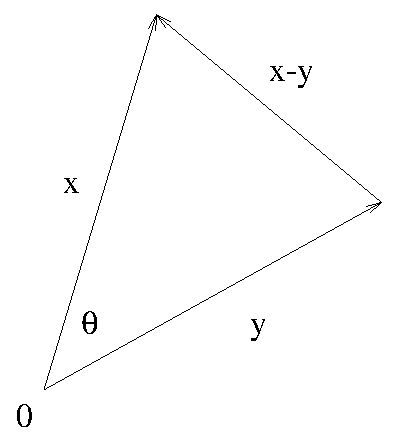
\psfig{file=../figures/costri.eps,height=2.0in}}
     \caption{Triangle formed by vectors $x$ and $y$ with interior
	angle $\theta$.}
     \label{F:costri}
\end{figure}

It follows from the law of cosines that
\[
||x-y||^2 = ||x||^2 + ||y||^2 - 2||x|| ||y||  \cos\theta.
\]
We claim that
\[
||x-y||^2 = ||x||^2 + ||y||^2 -2x\cdot y.
\]
Assuming that the claim is valid, it follows that
\[
x\cdot y = ||x|| ||y||  \cos\theta,
\]
which proves the theorem.  Finally, compute
\begin{eqnarray*}
||x-y||^2 & = &(x_1-y_1)^2 + \cdots + (x_n-y_n)^2 \\
& = & (x_1^2-2x_1y_1+y_1^2) + \cdots + (x_n^2-2x_ny_n+y_n^2)\\
& = & (x_1^2+\cdots+x_n^2)-2(x_1y_1+\cdots+x_ny_n)+(y_1^2+\cdots+y_n^2)\\
& = & ||x||^2 -2x\cdot y + ||y||^2
\end{eqnarray*}
to verify the claim.   \end{proof}

Theorem~\ref{T:dotangle} gives a numerically efficient method
for computing the angle\index{angle between vectors} between
vectors $x$ and $y$.  In \Matlab
this computation proceeds by typing
\begin{verbatim}
theta = acos(dot(x,y)/(norm(x)*norm(y)))
\end{verbatim} \index{\computer!acos}\index{\computer!dot}
where {\tt acos} is the inverse cosine of a number.
For example, using the $3$-vectors $x = (1,4,2)$ and $y =
(2,3,-1)$ entered previously, \Matlab responds with
\begin{verbatim}
theta =
    0.7956
\end{verbatim}
Remember that this answer is in radians\index{radians}.  To convert
this answer to degrees\index{degrees}, just multiply by $360$ and
divide by $2\pi$:
\begin{verbatim}
360*theta / (2*pi)
\end{verbatim}
to obtain the answer of $45.5847^\circ$.

\subsubsection{Area of Parallelograms}

Let $P$ be a parallelogram whose sides are the vectors $v$ and $w$ as
in Figure~\ref{F:parallel}.  Let $|P|$ denote the area of $P$.  As an
application of dot products \index{dot product} and
\eqref{e:dotproductang}, we calculate $|P|$. \index{parallelogram}
We claim that
\begin{equation}  \label{e:areaP}
|P|^2 = ||v||^2||w||^2 - (v\cdot w)^2.
\end{equation}
We verify \eqref{e:areaP} as follows.  Note that the area of $P$
is the same as the area of the rectangle $R$ also pictured in
Figure~\ref{F:parallel}.  The side lengths of $R$ are: $||v||$ and
$||w||\sin\theta$ where $\theta$ is the angle between $v$ and $w$.
A computation using \eqref{e:dotproductang} shows that
\begin{eqnarray*}
|R|^2 & = & ||v||^2 ||w||^2\sin^2\theta \\
& = & ||v||^2 ||w||^2(1-\cos^2\theta) \\
& = & ||v||^2 ||w||^2\left(1-\left(\frac{v\cdot w}{||v|| ||w||}
\right)^2\right)\\
& = & ||v||^2 ||w||^2 - (v\cdot w)^2,
\end{eqnarray*}
which establishes \eqref{e:areaP}.

\begin{figure}[htb]
     \centerline{%
     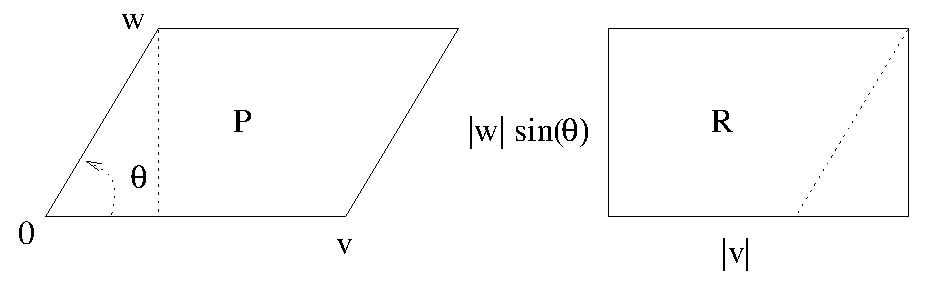
\psfig{file=../figures/parallel.eps,width=3.5in}}
     \caption{Parallelogram $P$ beside rectangle $R$ with same area.}
     \label{F:parallel}
\end{figure}


\EXER

\includeexercises
\end{document}
